\documentclass[12pt,a4paper]{article}
\title{%
  Øving 10 \\
  \large IELET1001 - Elektroteknikk \\
  }
\author{Gunnar Myhre, BIELEKTRO}

\usepackage[utf8]{inputenc}
\usepackage[norsk]{babel}
\usepackage[siunitx]{circuitikz}
\usepackage{amsmath}

\usepackage{pgfplots}
\pgfplotsset{compat=1.13}
\usepgfplotslibrary{fillbetween}

\usepackage{graphicx}
\graphicspath{ {./images} }

\setlength\parindent{0pt}

\begin{document}
  \maketitle

  \section*{Oppgåve 1}
    Oversetter verdiane til det komplekse domenet
    \begin{center}
      \begin{circuitikz}[american] \draw
        (0,0) to[I, l=$I_s$] (0,4) -- (2,4)
              to[R, l=4] (4,4)
              to[L, l=$j\omega5$] (4,0) -- (0,0)
        (2,4) to[C, l=$1/j\omega$, i=$I_o$] (2,2)
              to[R, l=4, v=$V_o$] (2,0)
        ;
      \end{circuitikz}
    \end{center}
    Finner $I_o$ vha. straumdeling
    \begin{equation}
      I_o = \frac{4+j\omega5}{8+j\left( \omega5 - \frac{1}{\omega} \right)}I_s
    \end{equation}
    finner $V_o$ vha. Ohms lov
    \begin{equation}
      V_o = 4I_o
    \end{equation}
    setter saman likningene og vinner uttrykk for transimpedansen $Z(j\omega)$
    \begin{equation}
      Z(j\omega) = \frac{V_o(j\omega)}{I_s(j\omega)} \rightarrow
      Z(j\omega) = \frac{16+j\omega20}{8+j\left( \omega5 - \frac{1}{\omega} \right) }
    \end{equation}

  \section*{Oppgåve 2}
    Oversetter verdiane til det komplekse domenet
    \begin{center}
      \begin{circuitikz}[american] \draw
        (0,0) to[V, l=$V_i$, invert] (0,3)
              to[R, l=$2$] (3,3)
              to[C, l=$5/j\omega$] (6,3)
              to[R, l=$5$, v=$V_o$] (6,0) -- (0,0)
        (3,3) to[C, l=$10/j\omega$] (3,0)

        (4,0) node[ground]{}
        (3,3) node[label={[font=\footnotesize]100:$V_2$}] {}
        (6,3) node[label={[font=\footnotesize]100:$V_o$}] {}
        ;
      \end{circuitikz}
    \end{center}
    Vi er ute etter transferfunksjonen $G_v(j\omega) = \frac{V_o(j\omega)}{V_i(j\omega)}$.
    Bruker nodespenning for å finne uttrykk for $V_o$ og $V_i$
    \begin{equation}
      KCL_{V_o}: 
      \frac{V_o - V_2}{5}j\omega + \frac{V_o}{5} = 0 \rightarrow
      V_2 = V_o + \frac{V_o}{j\omega}
    \end{equation}
    \begin{equation}
      KCL_{V_2}: 
      \frac{V_2 - V_i}{2} + \frac{V_2}{10/j\omega} + \frac{V_2-V_o}{5/j\omega} = 0
      \rightarrow V_2 = \frac{5V_i+2V_oj\omega}{5 + 3j\omega}
    \end{equation}
    setter saman likningene
    \begin{equation}
      \left(V_o + \frac{V_o}{j\omega}\right) \left( 5+3j\omega \right) = 5V_i + 2V_oj\omega
    \end{equation}
    forenkler algebraisk
    \begin{equation}
      5V_o + \frac{5V_o}{j\omega} + 3V_oj\omega + 3V_o -2V_oj\omega = 5V_i
    \end{equation}
    \begin{equation}
      8V_o + j\omega V_o + \frac{5}{j\omega}V_o = 5V_i
    \end{equation}
    \begin{equation}
      G_v(j\omega) = \frac{V_i(j\omega)}{V_o(j\omega)} = \frac{5}{8+j\omega + \frac{5}{j\omega}}
    \end{equation}
    her kan vi fjerne brøken i nemnaren ved å gonge med $\frac{j\omega}{j\omega}$




  \newpage

  \section*{Oppgåve 3}
    \begin{center}
      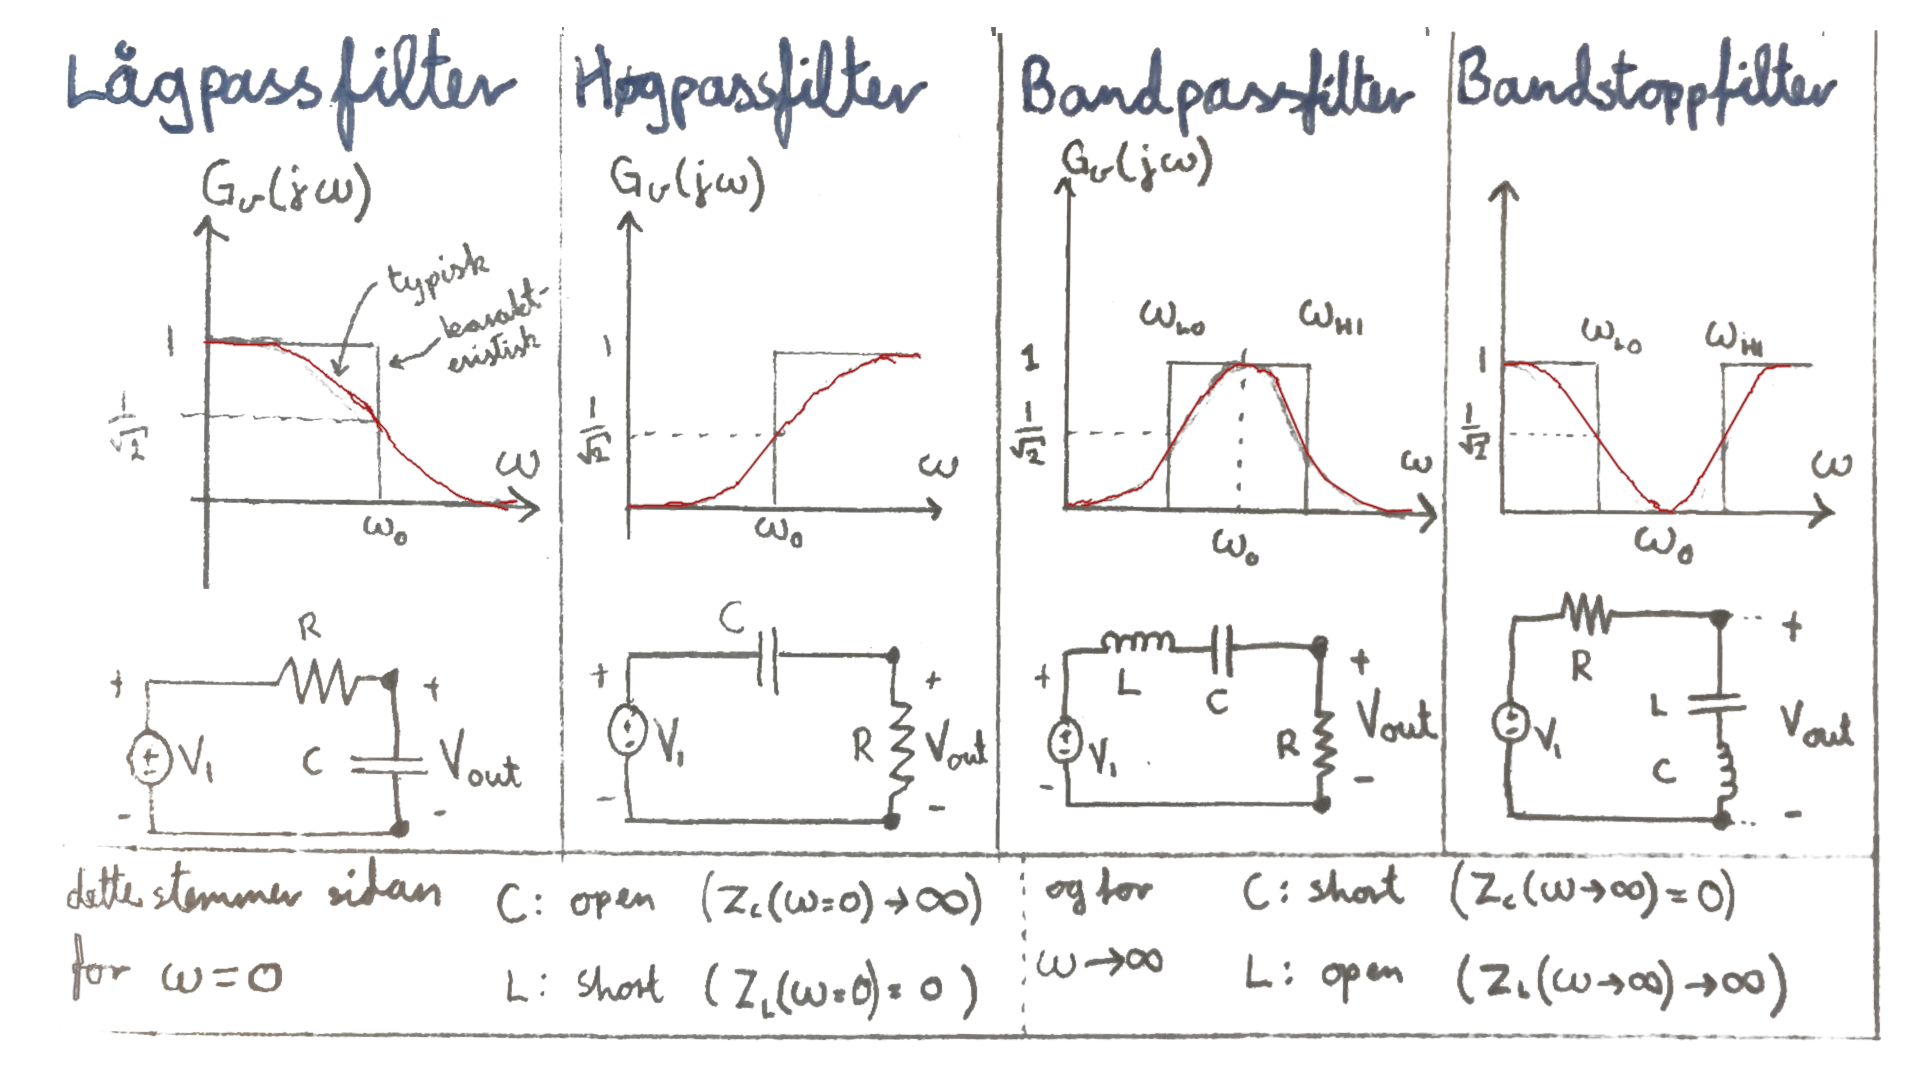
\includegraphics[scale=0.8]{10_filter.png}
    \end{center}
    I figuren over har eg teikna amplitudediagram og implementasjonseksempel
    for dei fire hovedtypane filter. Amplitudediagramma (øverste rad) er uttrykt ved
    transferfunksjonen for spenningsauke, $G_v(j\omega)$, langs y-aksa og vinkelfrekvensen $\omega$
    langs x-aksa. Den raude grafen representerer den typiske amplituden for eit filter av
    lågaste orden (første orden for låg- og høgpass, og andre orden for bandpass og bandstopp).
    Den grå, firkanta grafen representerer det karakteristiske eller \textit{ideelle} filteret.
    \begin{itemize}
      \item $\omega_o$ er resonansfrekvensen, og er å finne for alle
        filterkarakteristikkane.  Denne er bestemt som frekvensen der den
        totale reaktansen i filteret er null.
      \item $\omega_{LO}$ og $\omega_{HI}$ er knekkfrekvensar, eller
        \textit{cutoff}-frekvensar.  For alle filtertypene stemmer det at
        knekkfrekvensen er den/dei frekvensen/ane der halve effekten er
        overført frå innsignalet til utsignalet. For spenningsverdiar vert
        dette $\frac{1}{\sqrt{2}}G_v(j\omega)$. For lågpassfilter og
        høgpassfilter samanfaller knekkfrekvensen med resonansfrekvensen.
      \item Bandbredden er definert som intervallet mellom $\omega_{LO}$ og $\omega_{HI}$.
      \item Stoppbandet er frekvensintervallet der filteret stopper frekvensar,
        altså der $G_v(j\omega) \rightarrow 0$
      \item Passbandet er frekvensintervallet der filteret slepper igjennom
        frekvensar, altså der $G_v(j\omega) \rightarrow 1$
    \end{itemize}

  \section*{Oppgåve 4}
    \subsection*{a)}
    Vi kan sjå på formelen for impedans i spole i dei to ekstremtilfella
    \begin{itemize}
      \item $Z_L = j\omega L$
      \item $Z_L(\omega \rightarrow 0) \rightarrow 0$
      \item $Z_L(\omega \rightarrow \infty) \rightarrow \infty$
    \end{itemize}
    \begin{center}
      \begin{circuitikz}[american] \draw
        (0,3) to[R, l=$R_1$] (4,3)
              to[R, l=$R_2$, v=$V_o$] (4,0) -- (0,0)
        (0,3) to[open, v=$V_i$] (0,0)
        (1,3) -- (1,2) -- (3,2) -- (3,3)

        (7,3) to[R, l=$R_1$] (11,3)
              to[R, l=$R_2$, v=$V_o$] (11,0) -- (7,0)
        (7,3) to[open, v=$V_i$] (7,0)
        (8,3) to[short, -*] (8,2)
        (10,3) to[short, -*] (10,2)
        ;
      \end{circuitikz}
    \end{center}
    \begin{itemize}
      \item $\omega \rightarrow 0 \longrightarrow V_1 = V_o$
      \item $\omega \rightarrow \infty \longrightarrow V_o = \frac{R_2}{R_1 + R_2}V_i$
    \end{itemize}
    Sidan $R_1 >> R_2$ vil kretsen for $\omega \rightarrow \infty$ gjere at $G_v(j\omega)
    \rightarrow 0$. Det er med andre ord snakk om eit lågpassfilter.

  \subsection*{b)}
    Vi kan sette opp transferfunksjonen $G_v(j\omega)$ vha. formel for spenningsdeling.
    \begin{equation}
      G_v(j\omega) = \frac{V_o(j\omega)}{V_i(j\omega)} =
      \frac{R_2}{\frac{R_1j\omega L}{R_1 + j\omega L} + R_2}
    \end{equation}
    finner fellesnemnar for brøkane i nemnaren
    \begin{equation}
      \frac{R_2(R_1 + j\omega L)}{R_1j\omega L + R_2(R_1 + j\omega L)} \rightarrow
      \frac{R_1R_2 + R_2j\omega L}{R_1R_2 + R_1j\omega L + R_2 j\omega L}
    \end{equation}
    finner magnituden til $G_v$ ved å rekne modulen for begge dei komplekse tala
    \begin{equation}
      |G_v(j\omega)| = \frac{\sqrt{(R_1R_2)^2 + (R_2 \omega L)^2}}
      {\sqrt{(R_1R_2)^2 + (R_1\omega L + R_2 \omega L)^2}}
    \end{equation}
    Om vi setter inn for $\omega \rightarrow 0$ og $\omega \rightarrow \infty$ ser vi at
    denne modellen stemmer overeins med den kvalitative modellen i oppg. \textbf{a}.

  \section*{Oppgåve 5}
    \subsection*{a)}
    Impedansen til ein spole er gitt som
    \begin{equation}
      Z_L = j\omega L
    \end{equation}
    derfor vil impedansen gå mot null for $\omega \rightarrow 0$. I dette tilfellet vil
    $V_i = V_o$.

    \subsection*{b)}
    I tilfellet $\omega \rightarrow \infty$ vil impedansen til spolen gå mot
    uendeleg, altså som ein åpen krets.  Dermed vil utgongsspenninga gå mot $0V$

    \subsection*{c)}
    Ut ifrå denne karakteristikken kan vi slå fast at kretsen er eit lågpassfilter.

    \subsection*{d)}
    Finner fasevektorverdiar av dei oppgitte komponentverdiane
    \begin{itemize}
      \item $250mH \rightarrow Z_L = j\omega L = j\omega 250 \cdot 10^{-3}[\si{\ohm}]$
      \item $1,5\si{\kilo\ohm} \rightarrow Z_R = 1500[\si{\ohm}]$
    \end{itemize}
    Finner $V_o$ vha. spenningsdeling
    \begin{equation}
      V_o = \frac{R}{R+Z_L}V_i \rightarrow V_o = \frac{1500}{1500 + j\omega 0,25}V_i
    \end{equation}
    finner transferfunksjonen
    \begin{equation}
      G_v(j\omega) = \frac{V_i(j\omega)}{V_o(j\omega)} = \frac{1500}{1500+j\omega 0,25}
      \rightarrow G_v(j\omega) = \frac{6000}{6000 + j\omega}
    \end{equation}

    \subsection*{e)}
    For å finne knekkfrekvensen finner vi først magnituden til transferfunksjonen
    \begin{equation}
      |G_v(j\omega)| = \frac{\sqrt{6000^2}}{\sqrt{6000^2+\omega^2}}
    \end{equation}
    knekkfrekvensen finner vi når $G$ overfører halv effekt (merk at dette forholdet er
    $\frac{1}{\sqrt{2}}$ sidan vi snakker om spenning og ikkje effekt $P = \frac{V^2}{Z}$).
    \begin{equation}
      \frac{1}{\sqrt{2}} = \frac{\sqrt{6000^2}}{\sqrt{6000^2+\omega^2}}
      \rightarrow 6000^2 + \omega ^2 = 6000^2 \cdot 2
      \rightarrow \omega = 6000[rad/s]
    \end{equation}

    \subsection*{f)}
    Setter inn for oppgitte verdiar
    \begin{itemize}
      \item Knekkfrekvensen $\omega_c = 6000[rad/s]$
      \item $|G_v(j\omega)| = \frac{\sqrt{6000^2}}{\sqrt{6000^2+\omega^2}}$
      \item $|G_v(0,3\omega_c)| = 0,9486$
      \item $|G_v(\omega_c)| = 0,7071$
      \item $|G_v(3\omega_c)| = 0,5$
    \end{itemize}
    Desse kalkulasjonane viser at for lågare frekvensar vil overføringsfunksjonen mellom
    $V_i$ og $V_o$ gå mot 1, og for høgare frekvensar vil den gå mot 0.
    Dette stemmer overeins med antakelsen at kretsen er eit lågpassfilter.


  \section*{Oppgåve 6}
    \subsection*{a)}
    Komponentverdiane som fasevektorar er $Z_L = j\omega 0,05$ og $Z_R = 1000$.
    Vi kan finne $V_o$ vha. spenningsdeling.
    \begin{equation}
      V_o = \frac{j\omega 0,05}{1000 + j\omega 0,05}V_i
    \end{equation}
    som igjen lar oss finne overføringsfunksjonen
    \begin{equation}
      G_v(j\omega) = \frac{V_o}{V_i} = \frac{j\omega 0,05}{1000 + j\omega 0,05}
    \end{equation}
    vi kan se at for høge $\omega$ vil $G_v \rightarrow 1$, for låge $\omega$ vil
    $G_v \rightarrow 0$. Kretsen er eit høgpassfilter.

    \subsection*{b)}
    Finner først magnituden til $G_v$
    \begin{equation}
      |G_v(j\omega)| = \frac{\sqrt{(\omega 0,05)^2}}{\sqrt{1000^2 + (\omega 0,05)^2}}
    \end{equation}
    setter lik magnituden til knekkfrekvensen $\frac{1}{\sqrt{2}}$ og løyser for $\omega$
    \begin{equation}
      \frac{1}{\sqrt{2}} = \frac{\sqrt{(\omega 0,05)^2}}{\sqrt{1000^2 + (\omega 0,05)^2}}
      \rightarrow \omega ^2 (2\cdot 0,05^2 - 0,05^2) = 1000^2 
      \rightarrow \omega = 20000[rad/s]
    \end{equation}

    \subsection*{c)}
    Setter inn for oppgitte komponentverdiar
    \begin{itemize}
      \item $|G_v(j\omega)| = \frac{\sqrt{(\omega 0,05)^2}}{\sqrt{1000^2 + (\omega 0,05)^2}}$
      \item $\omega_c = 20000[rad/s]$
      \item $|G_v(0,1\omega_c)| = 0,0995$
      \item $|G_v(\omega_c)| = 0,7071$
      \item $|G_v(10\omega_c)| = 0,9950$
    \end{itemize}
    Desse kalkulasjonane stemmer overeins med at kretsen er eit høgpassfilter. For låge
    frekvensar er magnituden til overføringsfunksjonen liten, for høge frekvensar er
    den stor.

  \section*{Oppgåve 7}
    Vi har lært at resonansfrekvensen til eit bandpass-/bandstoppfilter kan
    finnast på denne måten dersom vi kjenner knekkfrekvensane:
    \begin{equation}
      \omega_{LO}\cdot\omega_{HI} = \omega_0^2 \rightarrow
      \omega_0 = \sqrt{\omega_{LO}\omega_{HI}} = 189,7[rad/s]
    \end{equation}
    bandbredda er intervallet mellom dei to knekkfrekvensane
    \begin{equation}
      \omega_{HI} - \omega_{LO} = 20[rad/s]
    \end{equation}
    kvalitetsfaktoren kan vi finne på denne måten
    \begin{equation}
      Q = \frac{\omega_0}{BW} = 3\sqrt{10} \approx  9,5
    \end{equation}

  \section*{Oppgåve 8}
    \subsection*{a)}
    Oppførselen ved ekstremverdiane kan vi finne i formlane for impedans i spole og
    kondensator
    \begin{itemize}
      \item $Z_L = j\omega L, Z_L(\omega \rightarrow 0) \rightarrow 0,
        Z_L(\omega \rightarrow \infty) \rightarrow \infty$
      \item $Z_C = \frac{1}{j\omega C}, Z_C(\omega \rightarrow 0) \rightarrow \infty,
        Z_C(\omega \rightarrow \infty) \rightarrow 0$
    \end{itemize}

    \subsection*{b)}
    Impedansen til parallellkoplinga er gitt som
    \begin{equation}
      Z = \frac{j\omega L/j\omega C}{\frac{1}{j\omega C} + j\omega L} =
      \frac{L/C}{j(\omega L - \frac{1}{\omega C})}
    \end{equation}

    \subsection*{c)}
    Vi ser at dersom nemnaren går mot null vil impedansen skyte i været. Dette er
    resonansfrekvensen. Denne kan vi finne slik:
    \begin{equation}
      \left(\omega L - \frac{1}{\omega C}\right) = 0 \rightarrow \omega ^2 = \frac{1}{LC}
      \rightarrow \omega = \omega_0 = \frac{1}{\sqrt{LC}}
    \end{equation}
    vi kan sette inn for resonanfrekvensen $\omega_0$ i formelen for impedansen i parallell
    \begin{equation}
      Z_{max} = \frac{L/C}{j(\frac{L}{\sqrt{LC}} - \frac{\sqrt{LC}}{C})} =
      \frac{L/C}{\frac{LC}{\sqrt{LC}C} - \frac{LC}{\sqrt{LC}C}} = 0
    \end{equation}
    utgongsspenninga i resonanstilfellet vert
    \begin{equation}
      V_o = \frac{R}{R + Z_{max}}V_i \longrightarrow
      V_o = \frac{R}{R}V_i = V_i
    \end{equation}

    \subsection*{d)}
    For høge eller låge frekvensar vil impedansen i parallellkoplinga gå mot null, og dermed
    vil $V_i = V_o$. Det er dermed snakk om eit bandpassfilter.


    \begin{center}
      \pgfmathdeclarefunction{normalcurve}{0}{\pgfmathparse{1*1/exp(((x-3)^2)/2)}}
      \begin{tikzpicture}
        \begin{axis}[xlabel=$\omega$, ylabel=$|G_v(j\omega)|$,
                xlabel style={at=(current axis.right of origin), anchor=west},
                ylabel style={at=(current axis.above origin), anchor=south},
                ymin = 0, ymax=1.1, axis x line = bottom, axis y line=middle,
                xtick={3},
                xticklabels={$\omega_0$},
                 legend pos=outer north east]
        \addplot [name path=A, domain=0:6,cyan, thick, samples=150] {normalcurve};
        \draw[dashed] (3,1) -- (3,0);
        \node at (3,1) {\textbullet};
        \end{axis}
      \end{tikzpicture}
    \end{center}


  \section*{Oppgåve 9}
    \subsection*{a)}
    Setter opp KCL i inputnodene til OP-ampen. Vi veit at spenninga desse nodene
    er lik, og kaller den $V_1$
    \begin{itemize}
      \item $(V_1 - V_s)j\omega C + \frac{V_1}{9000} = 0 \rightarrow
        V_1 = \frac{V_sj\omega C}{j\omega C + 9000^{-1}}$
      \item $\frac{V_1}{R_1} + \frac{V_1 - V_o}{R_2} = 0 \rightarrow
        V_1 = \frac{V_oR_1}{R_1 + R_2}$
    \end{itemize}
    setter saman for $V_1$
    \begin{equation}
        \frac{V_sj\omega C}{j\omega C + 9000^{-1}} = \frac{V_oR_1}{R_1 + R_2}
        \rightarrow \frac{V_o}{V_s} = \frac{j\omega C(R_1 + R_2)}{R_1(j\omega C + 9000^{-1})}
    \end{equation}

    \subsection*{b)}
    Finner først magnituden til $G_v$
    \begin{equation}
      |G_v(j\omega)| = \frac{R_1\omega C + R_2\omega C}
      {\sqrt{\left(\frac{R_1}{9000}\right)^2 + (R_1\omega C)^2}}
    \end{equation}
    Vi ønsker at forsterkinga skal vere $4$ for høge frekvensar. For høge frekvensar
    er alle ledda uten $\omega$ irrelevante.
    \begin{equation}
      4 = \frac{R_1\omega C + R_2 \omega C}{R_1 \omega C}
    \end{equation}
    vi har opplyst at $R_1 = 10\si{\kilo\ohm}$
    \begin{equation}
      4 = \frac{10^4 + R_2}{10^4} \rightarrow R_2 = 30\si{\kilo\ohm}
    \end{equation}
    Det er også spesifisert ein knekkfrekvens $f_c = 4kHz \rightarrow \omega_c = 8000\pi[rad/s]$.
    Vi veit at knekkfrekvensen opptrer når den overførte effekten er halvparten av
    maksimumnivået. Dette kan vi formulere slik:
    \begin{equation}
      |G_v(j\omega_c)| = \frac{4}{\sqrt{2}}
    \end{equation}
    Setter inn for dei kjente mengdene i $|G_v|$ og finner $C$
    \begin{equation}
      \frac{4}{\sqrt{2}} = \frac{(10^4\cdot 8000\pi + 3\cdot 10^4 \cdot 8000 \pi)C}
      {\sqrt{\frac{100}{81} + 6,4\cdot 10^{15} \pi^2C}} \rightarrow
      C^2 = \frac{800/81}{10,24\cdot10^{10}\pi^2 - 8\cdot6,4\cdot 10^{15}\pi^2}
    \end{equation}
    Finner $C = j4,421 \cdot 10^{-9} \rightarrow C = 4,421[\si{\nano\farad}]$. Eg forventa ikkje
    å få eit imaginært svar så eg er ikkje sikker på kva dette skyldast, men det har nok å gjere
    med at transferfunksjonen tar in ein imaginær verdi $G_v(\textbf{j}\omega)$.


  \section*{Oppgåve 10}
    Setter opp KCL i inputnoda til OP-ampen. Her er spenninga $0V$ sidan den eine
    noda er kopla til jord.
    \begin{equation}
      \frac{-V_i}{R_1 + 1/j\omega C_1} +
      \frac{-V_o}{\frac{R_2\cdot 1/j\omega C_2}{R_2 + 1/j\omega C_2}} = 0
      \rightarrow \frac{V_o}{V_i} = -\frac{R_2\cdot 1/j\omega C_1}
      {\left( R_1 + \frac{1}{j\omega C_1} \right) \left( R_2 + \frac{1}{j\omega C_2} \right)}
    \end{equation}
    Amplitudekarakteristikken kan vi antyde slik: Når vinkelfrekvensen går mot null
    oppfører $C_1$ seg som ein åpen krets og $V_i$ er derfor avkopla kretsen. Når
    vinkelfrekvensen går mot uendeleg oppfører $C_2$ seg som ein kortslutning, dermed er det
    spenninga frå inngongen på OP-ampen ($0V$) som står på $V_o$.
    \begin{center}
      \begin{tabular}{|c|c|}
        \hline
         & \\
        vinkelfrekvens & overføringsfunksjon $|G_v(j\omega)|$ \\
         & \\
        \hline
        $\omega \rightarrow 0$ & 0 \\
        \hline
        $\omega \rightarrow \infty$ & 0 \\
        \hline
      \end{tabular}
    \end{center}
    For å finne resonansfrekvensen separerer eg den reelle og imaginære delen av 
    overføringsfunksjonen
    \begin{equation}
      G_v(j\omega) = - \frac{R_2 \cdot 1/j\omega C_1}
      {R_1R_2 - \frac{1}{\omega^2C_1C_2} + \frac{R_1}{j\omega C_2} + \frac{R_2}{j\omega C_1}}
      \rightarrow G_v(j\omega) = 
      - \left[ \frac{1}{j\omega C_1R_1} + \frac{R_2}{R_1}\frac{C_2}{C_1}
      + 1 + jR_2\omega C_2 \right]
    \end{equation}
    resonansfrekvensen opptrer når den totale reaktansen er null, så vi setter den imaginære
    delen av likninga over lik null
    \begin{equation}
      \frac{1}{j\omega C_1R_1} + jR_2\omega C_2 = 0 \rightarrow
      \omega ^2 = \frac{1}{R_1R_2C_1C_2} \rightarrow
      \omega = \omega _0 = \frac{1}{\sqrt{R_1R_2C_1C_2}}
    \end{equation}
    finner først magnituden til $G_v$
    \begin{equation}
      |G_v(j\omega)| = - \left[ \frac{R_2 \cdot\frac{1}{\omega C_1}}
      {\sqrt{ \left(R_1R_2 - \frac{1}{\omega ^2 C_1C_2} \right)^2 +
              \left(\frac{R_1}{\omega C_2} + \frac{R_2}{\omega C_1} \right)^2}} \right]
    \end{equation}
    setter vi inn for $\omega = \omega _0 = \frac{1}{\sqrt{R_1R_2C_1C_2}}$ i dette uttrykket
    finner vi forsterkinga ved resonansfrekvensen.

    \bigskip

    Filteret er eit invertert bandpassfilter, sidan låge og høge frekvensar vert
    attenuert og eit område i midten har negativ forsterking.

\end{document}
